\chapter{Point estimators and parametric models}

%\section{What does learning mean and why is it interesting?}
%\todo{what is learning?}
%\todo{general overview over this chapter}
%\todo{explain bias and consistency}
% \section{Motivation for learning DPPs}

Parameter estimation is one of the central components of every theory of real world phenomena. In a nutshell one could split the process of the construction of a descriptive model into two parts. The first one being the selection of the model which is done by a scientist and the second being the determination of the constants that belong to the model.

To make this more clear we will consider one of the most famous advances in the natural sciences namely the law of universal gravitation that was discovered by Sir Isaac Newton\todo{cite}. More precisely Newton discovered that the gravitational force acting between two massive objects is given by
\[F = G\cdot \frac{m_1m_2}{r^2}\]
where \(m_1, m_2\) are the masses of the two objects, \(r\) is the distance of the centers of masses and \(G\) is the gravitational constant. This constant can not be deduced from the theory itself and needs to be estimated based on some empirical data.

If we want to describe, simulate and predict the occurence of diverse subsets we can take a similar approach and impose the model of a determinantal point process. % which would correspond to the first part
This will usually be an assumption that will not strictly hold, but will often lead to reasonable, sometimes even impressive results. We will not be concerned in a measure of how justifiable this model selection is, although this is a highly interesting question and there exist ways to deal with it\todo{cite paper about KL divergence}. Leaving that aside we are left with the second step, namely the estimation of the parameters of the model, which are in the case of a DPP over a set of cardinality \(N\) exactly \(N(N-1)/2\). Because of the rather large amount of parameters and also the complicated structure of the DPPs it will in practice only be possible to perform those estimations through the use of computational tools. The task of computer based parameter or density estimation is an important field in the discipline of \emph{machine learning} and thus we will sometimes speak of the parameters being learned instead of estimated. Actually the interest of parameter estimation for DPPs arose from the machine learning community at the beginning of this decade. However we will phrase things in a way that no prior knowledge in this field is required.

In this chapter we will be concerned in how we can make point estimates for either the marginal or the elementary kernels \(K\) and \(L\). Point estimators are the most basic type of estimators and consist of the suggestion of one possible parameter set, for example in the case of the gravitational constant 
\[6.674\cdot10^{-11}\si{N.kg^{-2}.m^2}. \]
This is in contrast to the Bayesian approach to parameter estimation that we will present in the next chapter where the philosophy is to estimate a distribution over all possible parameter sets that indicates how likely they are given some the empirical data. We will discuss two essentially different methods of point estimators, the first one provides a way to reconstruct a marginal kernel for the empirical marginal distributions at least in the case where the empirical distribution is essentially a DPP. The other type of methods are all maximum likelihood estimators in different variations. 

But before we can proceed we want to remind the reader of two desirable properties of point estimators. For this we will assume that we want to estimate the distribution of a random variable \(X\) from a parametric family of probability measures
\[\left\{ \mathbb P_\theta\mid \theta\in\Theta\right\}.\]
This means we want to estimate \(\theta\) out of a possible set of parameters \(\Theta\) such that \(X\) is distributed according to \(\mathbb P_\theta\) which we will based upon some data \(x_1, \dots, x_n\). Further we assume that those points are actually generated by \(\mathbb P_\theta\) for one \(\theta\in\Theta\) and denote the estimator by \(\hat\theta_n\). We call \emph{unbiased} if we have
\[\mathbb E[\hat\theta_n] = \theta\]
and \emph{consistent} if we have
\[\hat\theta_n\to\theta \quad \text{in probability}.\]

It shall be noted that although those properties are beneficial, they are not crucial for an estimator to be reasonable. First they both assume that the data generating process, i.e. the process one wants to describe actually follows one of the laws \(\mathbb P_\theta\) which will typically be not the case in real world examples. Further the asymptotic property of consistency is rather of theoretical nature since in practice it is not possible to create large sets of empirical data and certainly not infinitely large ones. 

%In practice this will be a rather large amount of parameters and therefore it will only be possible

\section{Reconstruction of the marginal kernel using principal minors} %  via the Assymptotic reconstruction of the kernel}

%In this section we want to see how we can estimate the marginal kernel from an increasing number of observations \(\mathbf Y_1, \dots, \mathbf Y_n\subseteq \mathcal Y\) that are distributed according to \(\mathbb P\). For this we will sketch the procedure in \cite{urschel2017learning}. 
Now we will display the first way how one can estimate the marginal kernel \(K\) of a DPP based on some samples drawn from it.

\begin{emp}[Setting]
Let \(\mathcal Y\) be a finite set of cardinality \(N\) and let \(K\in\mathbb R^{\mathcal Y\times\mathcal Y}_{\text{sym}}\) satisfy \(0\le K\le I\). Let further \(\mathbf Y_1, \mathbf Y_2, \dots\) be distributed according to the DPP with marginal kernel \(K\).
\end{emp}

In order to perform an approximate reconstruction of the marginal kernel we will need to consider the \emph{empirical measure} % \(\hat{\mathbb P}_n\) be 
\[\hat{\mathbb P}_n \coloneqq \frac1n\sum_{i=1}^n\delta_{\mathbf Y_i}.\]
% We can identify the probability measures on a finite set, in our case \(2^{\mathcal Y}\), with the probability simplex
% \[\left\{ x\in\mathbb R^{2^{\mathcal Y}} \;\Big\lvert\; x_A \in[0, 1] \text{ for all } A\in 2^{\mathcal Y} \text{ and } \sum_{A\in 2^{\mathcal Y}} x_A = 1 \right\}.\]
The interest in \(\hat{\mathbb P}_n\) lies in the fact that they quite natural estimates for the actual underlying distribution. 
% It is well known that \(\hat{\mathbb P}_n\) 
More precisely they are {unbiased estimators} for \(\mathbb P\), i.e. they agree in expectation with \(\mathbb P\). This can be seen by evaluating it at \(A\subseteq \mathcal Y\)
\[\mathbb E_{\mathbb P}\big[\hat{\mathbb P}_n(A)\big] =\frac1n \sum_{i = 1}^n \mathbb E_{\mathbb P}\big[\delta_{\mathbf Y_i}(A)\big] =  \mathbb P(A).\]
And even stronger by the strong law of large numbers they converge to \(\mathbb P\) almost surely if the sequence \((\mathbf Y_k)_{k\in\mathbb N}\) of observations is independent. This can be seen by identifying the probability measures on \(2^{\mathcal Y}\) with the probability simplex
\[\left\{ \mu\in\mathbb R^{2^{\mathcal Y}} \;\Big\lvert\; \mu_A\in[0, 1] \text{ for all } A\subseteq\mathcal Y \text{ and } \sum_{A\subseteq\mathcal Y}\mu_A = 1 \right\}\]
and using the strong law of large numbers in \(\mathbb R^{2^{\mathcal Y}}\).

Therefore the empirical measures are reasonable approximations of the actual probability distribution. Assume now for one moment that the empirical measures \(\hat{\mathbb P}_n\) are also determinantal point processes with marginal kernel \(\hat K_n\), then \(\hat K_n\) would be a quite intuitive estimate for the actual marginal kernel \(K\). Thus we are interested in the question whether we can reconstruct the kernel marginal of a DPP if we know the DPP itself. Since the marginal density of a DPP corresponds to the principal minors of the marginal kernel, we first investigate whether we can reconstruct a matrix from its principle minors. For the answer to this problem we follow the main ideas presented in \cite{urschel2017learning} and \cite{rising2015efficient} although we modify their arguments to make them shorter and hopefully more accessible. \todo{say something about stability?}


%Therefore we can consistently %\todo{explain consistency}{ } 
%estimate all principal minors of \(K\), since
%\[\hat{\mathbb P}_n(A\subseteq \mathbf Y) \xlongrightarrow{n\to\infty} \mathbb P(A\subseteq\mathbf Y) = \det(K_A) \quad \text{almost surely}.\]


%Assume that \(\hat{\mathbb P}_n\) is a DPP with marginal kernel \(\hat K_n\), then \(\hat K_n\) would be a quite natural estimate for the actual marginal kernel \(K\).
%To make this approach rigorous we have to convince ourselves that the empirical measure are in fact DPPs and that a marginal kernel can be reconstructed from the DPP.

%it is natural to ask whether we can reconstruct the kernel 



% Thus the question naturally arrises whether we can reconstruct the kernel \(K\) from the knowledge of all of its principal minors, which we will address in the following.

%\subsubsection*{The principal minor assignment problem}\todo{phrase it very clearly}
\todo{define principle minors?}
\begin{emp}[The principal minor assignment problem]
Let \(K\in\mathbb R^{N\times N}\) be a symmetric matrix. We want to investigate whether \(K\) uniquely specified by its principle minors
\[\Delta_S \coloneqq \det(K_S) \quad \text{where } S\subseteq\left\{ 1, \dots, N\right\}.\]
We call this the \emph{symmetric principal minor assignment problem} and it will turn out that the matrix \(K\) can be reconstructed up to an equivalence relation.
\end{emp}

%The reconstruction of a symmetric matrix from all its principal minors is known as the \emph{principal minor assignment problem} and we aim to prove in this section that this is possible -- at least up to an equivalence relation. 
Before we present the general procedure we want to see how this would work in the case of a symmetric \(3\times3\) matrix \(K = (K_{ij})_{1\le i, j\le 3}\). First we note that we can regain the diagonal elements as the determinant of the \(1\times1\) principal minors
\[\det(K_{\left\{ i\right\}}) = K_{ii} \quad \text{for } i = 1, 2, 3.\]
Further the squares of the off diagonal are determined by the \(2\times2\) principal minors since
\[\det(K_{\left\{ i, j\right\}}) = K_{ii}K_{jj} - K_{ij}^2 \quad \text{for }i, j = 1, 2, 3.\]
Therefore we only need to reconstruct the signs off diagonal entries. To do this, we consider the determinant of the matrix itself
\begin{equation}\label{thrtimthr}
\det(K) = K_{11}K_{22}K_{33} + 2K_{12}K_{13}K_{23} - K_{11}K_{23}^2 - K_{22}K_{13}^2 - K_{33}K_{12}^2.
\end{equation}
Rearranging this yields
\[K_{12}K_{13}K_{23} = \frac12\left( \det(K) + K_{11}K_{23}^2 + K_{22}K_{13}^2 + K_{33}K_{12}^2 - K_{11}K_{22}K_{33}\right).\]
Since we know all of the expressions on the right side, we can determine the sign of the product on the left side. Now we assign the the signs of the off diagonal elements in such a way, that the above equation holds. More precisely if the the product is negative, we assign a minus to one or all three elements, if it is positive, then we assign a minus to none or two elements. If the product is zero, every configuration of signs satisfy the desired property. It is now straight forward to check that this assignment actually leads to the desired principle minors.
% \todo{explain this.}


\begin{emp}[Notions from graph theory]
In order to generalise the procedure above to larger matrices we will need some elementary concepts from graph theory. For this let \(G = (V, E)\) be a finite graph, i.e. \(V\) is a finite set, called the \emph{vertex set} and \(E\) consists of subsets of \(V\) with two elements, the \emph{edges}. Sometimes we will be sloppy in notation and not distinguish between the graph and the edge set. We will need the following notions:
\begin{enumerate}
\item \emph{Degree:} For a vertex \(v\in V\) the \emph{degree} is the number of edges that contains \(v\). 
\item \emph{Subgraph:} A graph \(\tilde G = (\tilde V, \tilde E)\) is called a \emph{subgraph} of \(G\) if \(\tilde V\subseteq V\) and \(\tilde E\subseteq E\).
\item \emph{Induced graph:} For a subset \(S\subseteq V\) of vertices the \emph{induced graph} \(G(S) = (S, E(S))\) is formed of all edges \(e\in E\) of \(G\) that are subsets of \(S\).
\item \emph{Path:} A \emph{path} in \(G\) is a sequence \(v_0v_1\cdots v_k\) of vertices such that \(\left\{ v_{i-1}, v_{i}\right\}\in E\) for all \(i = 1, \dots, k\).
\item \emph{Connected graph:} A graph is called \emph{connected} if for every pair of vertices \(v, w\in V\) there is a path from \(v\) to \(w\).
%, i.e. there is a sequence \(\left\{ v, v_1\right\}, \left\{ v_1, v_2\right\}, \dots, \left\{ v_{k-1}, v_k\right\}, \left\{ v_k, w\right\}\) of edges.
\item \emph{Cycle:} A \emph{cycle} \(C\) is a connected subgraph such that every vertex has even degree in \(C\). 
\item \emph{Cycle space:} Each cycle \(C\) can be identified with a vector \(x = x(C)\in\mathbb F_2^{E}\) such that
\[x_e\coloneqq \begin{cases} 1 \quad & \text{if } e\in C \\ 0 \quad & \text{if } e\notin C\end{cases}\]
indicates whether the edge \(e\in E\) belongs to the cycle \(C\). The \emph{cycle space} \(\mathcal C\) is the span of \(\left\{ x(C)\mid C\text{ is a cycle}\right\}\) in \(\mathbb F_2^{E}\). Note that the sum of two cycles in the cycle space corresponds to the symmetric difference of the edges.
%\item \emph{Simple cycle:} A cycle is called \emph{simple} if every vertex of \(C\) has even degree in \(C\).
%\item \emph{Cycle basis:} A basis of the cycle space is called \emph{cycle basis} if it consists of simple cycles.
\item \emph{Chordless cycle:} A cycle \(C\) is called \emph{chordless} if two verteces \(v, w\in C\) form an edge in \(G\) if and only they form an edge in \(C\). This is equivalent to the statement that \(C\) is an induced subgraph that is a cycle.
\item \emph{Cycle sparsity:} The cycle sparsity is the minimal number \(l\) such that a basis of the cycle space consisting of chordless cycles exists. Such a basis is called \emph{shortest maximal cycle basis} or short \emph{SMCB}. If the cycle space is trivial we define the cycle sparsity to be \(2\).
\item \emph{Pairings:} Let \(S\subseteq V\) be a set of of vertices. Then a \emph{pairing} \(P\) of \(S\) is a subset of edges of \(G(S)\) such that two different edges of \(P\) are disjoint. The vertices contained in the edges of \(P\) are denoted by \(V(P)\) and the set of all pairings by \(\mathcal P(S)\).
\end{enumerate}
\end{emp}\todo{add pictures and explanations?}

In order to see that the above definition of the cycle sparsity is well defined, we have need to show that shortest maximal cycle basis exist. This might be well known to people that are familiar with graph theory, but we will present an elementary proof here. It shall be noted, that the proof -- and also the definitions above -- becomes quite a lot more intuitive by drawing the according cycles in order to understand how the respective decompositions of cycles work.

\begin{prop}[Existence of SMCBs]
There always exists a basis \(\left\{ x(C_1), \dots, x(C_k)\right\}\) of the cycle space where \(C_1, \dots, C_k\) are chordless cycles.
\end{prop}
\begin{proof}
First we prove that the set of simple cycles generates the whole cycle space which we can then improve to show that the simple chordless cycles already generate the cycle space. A shortest maximal cycle basis is then attained by successively dropping simple chordless cycles.

We show that every cycle \(x(C)\) can be written as the sum of simple cycles \(x(C_1), \dots, x(C_k)\) where \(C_i\subseteq C\). This is equivalent to the statement that the edges of every cycle are the disjoint union of the edges of simple cycles. Take now a maximal non intersecting path \(v_0v_1\cdots v_k\).
\begin{figure}[h!]\label{makesimple}
	\centering
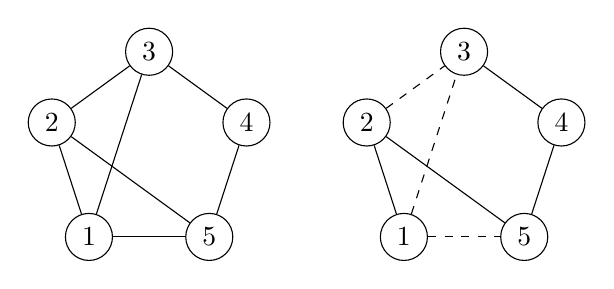
\begin{tikzpicture}%[shorten >=1pt,->]

  \tikzstyle{vertex}=[draw,circle,minimum size=17pt,inner sep=0pt]

  \foreach \name/\angle/\text in {A-1/234/1, A-2/162/2, 
                                  A-3/90/3, A-4/18/4, A-5/-54/5}
    \node[vertex,xshift=5cm,yshift=.5cm] (\name) at (\angle:1.3cm) {\(\text\)};
    
  \foreach \name/\angle/\text in {B-1/234/1, B-2/162/2, 
                                  B-3/90/3, B-4/18/4, B-5/-54/5}
    \node[vertex,xshift=9cm,yshift=.5cm] (\name) at (\angle:1.3cm) {\(\text\)};

  \foreach \from/\to in {1/2,2/3,3/4,4/5,5/1,1/3,5/2}
    \draw (A-\from) -- (A-\to);

\foreach \from/\to in {1/2,2/5,5/4,4/3}
\draw (B-\from) -- (B-\to);
\foreach \from/\to in {1/3,2/3,1/5}
\draw[dashed] (B-\from) -- (B-\to);
\end{tikzpicture}
\caption{Illustration of the search for a simple cycle in a graph with degrees greater than two. Once a maximal non intersecting path like \(12543\) is selected, every continuation of the path -- in this case 2 or 1 -- is already present in the path and therefore induces a simple cycle.}
\end{figure}
Since \(v_k\) has degree at least \(2\), there is an edge \(\left\{ v_k, v_{k+1}\right\}\) such that \(v_{k+1}\ne v_{k-1}\). Since the path is maximal, \(v_{k+1}\) has to agree with one a vertex \(v_i\in\left\{ v_0, \dots, v_{k-2}\right\}\), because otherwise we could add \(v_{k+1}\) to the path which is a contradiction to the maximality. Now \(v_iv_{i+1}\cdots v_kv_i\) corresponds to a simple cycle \(C_1\) and \(C_2\coloneqq C\setminus C_1\) is again a cycle. Thus we can write \(C\) as the disjoint union \(C = C_1\cup C_2\) where \(C_1\) is a simple cycle. By repeating this procedure we get the desired expression for \(C\) in terms of simple cycles.

To prove that already the simple chordless cycles generate the cycle space we have to prove that we can write every simple cycle \(x(C)\) as a sum of simple chordless cycles \(x(C_1), \dots, x(C_k)\). Let \(\left\{ \left\{ v_0, v_1\right\}, \dots, \left\{ v_k, v_0\right\}\right\}\) be the edge set of \(C\) and assume that \(C\) is not chordless like in Figure \ref{makechordless}, otherwise the statement would be trivial.
\begin{figure}[h!]\label{makechordless}
	\centering
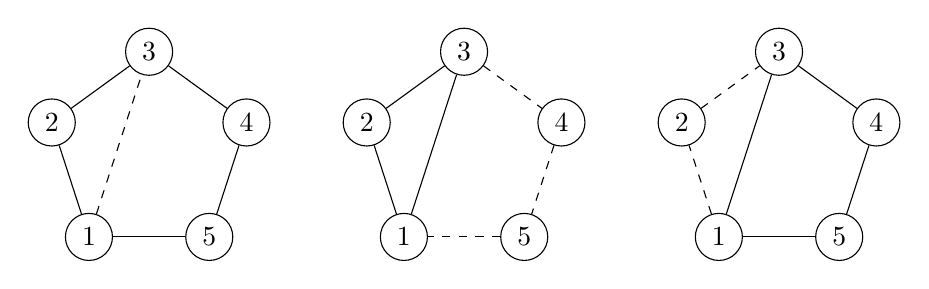
\begin{tikzpicture}%[shorten >=1pt,->]

  \tikzstyle{vertex}=[draw,circle,minimum size=17pt,inner sep=0pt]

  \foreach \name/\angle/\text in {A-1/234/1, A-2/162/2, 
                                  A-3/90/3, A-4/18/4, A-5/-54/5}
    \node[vertex,xshift=5cm,yshift=.5cm] (\name) at (\angle:1.3cm) {\(\text\)};
    
  \foreach \name/\angle/\text in {B-1/234/1, B-2/162/2, 
                                  B-3/90/3, B-4/18/4, B-5/-54/5}
    \node[vertex,xshift=9cm,yshift=.5cm] (\name) at (\angle:1.3cm) {\(\text\)};

  \foreach \name/\angle/\text in {C-1/234/1, C-2/162/2, 
                                  C-3/90/3, C-4/18/4, C-5/-54/5}
    \node[vertex,xshift=13cm,yshift=.5cm] (\name) at (\angle:1.3cm) {\(\text\)};

  \foreach \from/\to in {1/2,2/3,3/4,4/5,5/1}
    \draw (A-\from) -- (A-\to);
\draw[dashed] (A-1) -- (A-3);

\foreach \from/\to in {1/2,2/3,3/1}
\draw (B-\from) -- (B-\to);
\foreach \from/\to in {3/4,4/5,5/1}
\draw[dashed] (B-\from) -- (B-\to);

\foreach \from/\to in {1/2,2/3}
\draw[dashed] (C-\from) -- (C-\to);
\foreach \from/\to in {1/3,3/4,4/5,5/1}
\draw (C-\from) -- (C-\to);
\end{tikzpicture}
\caption{The simple cycle \(123451\) on the left is not chordless but the symmetric difference of the two simple chordless cycles \(1231\) and \(13451\) on the right.}
\end{figure}
 Thus there is are indices \(1\le i<j-1\le k-1\) such that \(\left\{ v_i, v_j\right\}\in E\). Let now \(C_1\) and \(C_2\) be the two cycles associated with the paths
\[v_0v_1 \cdots v_iv_jv_{j+1}\cdots v_kv_0\quad \text{and } v_iv_{i+1}\cdots v_{j-1}v_jv_i.\]
Then we have \(x(C) = x(C_1) + x(C_2)\). By iterating this procedure as long as the cycles are not chordless the desired decomposition can be achieved in finitely many steps.

%Since we have defined the cycle space as the span of all vectors \(x(C)\) where \(C\) is a cycle, it suffices to show that every cycle \(C\) admits a decomposition
%\[x(C) = x(C_1)+\dots+x(C_m)\]
%where \(C_1, \dots, C_m\) are chordless cycles. If \(C\) is already chordless, then we are done, so we can assume that the vertices of \(C\) are \(\left\{ v_1, \dots, v_M\right\}\) with\todo{finish this proof!}
\end{proof}\todo{cite the theorem with its actual name}

\begin{defi}[Determinantal equivalence]
Two symmetric matrices \(A, B\in\mathbb R^{N\times N}\) are called \emph{determinantally equivalent} if the have the same principal minors and we write \(A\sim B\).
\end{defi}

It is obvious that we can only hope to reconstruct a symmetric matrix up to determinantal equivalence. However this would be satisfactory, because determinantally equivalent matrices are exactly those that give rise to the same DPP. Let us in the following denote the principal minor \(\det(K_S)\) by \(\Delta_S\) for \(S\subseteq\left\{ 1, \dots, N\right\}\). To come back to our original problem, we notice that the principal minors up to size two immediately determine the diagonal and the absolute values of the off diagonal of \(K\) since we have
\begin{equation*}\label{e3.0}
K_{ii} = \Delta_{\left\{ i\right\}} \quad \text{and } K_{ij}^2 = K_{ii}K_{jj} - \Delta_{\left\{ i, j\right\}}.
\end{equation*}
Thus it only remains to regain the signs \(\operatorname{sgn}(K_{ij})\) of the off diagonal entries. For this we use the following object.

\begin{emp}[The adjacency graph and sign function]
The adjacency graph \(G_K = (V_K, E_K)\) associated with \(K\) consists of the vertex set \(\left\{ 1, \dots, N\right\}\) and \(\left\{ i, j\right\}\) form an edge if and only if \(K_{ij}\ne0\). Further we introduce some \emph{weights} on the edges. This means we consider a mapping \(w\colon E_K\to\mathbb R\) and we set
\[w_{ij} \coloneqq w(\left\{ i, j\right\}) \coloneqq \operatorname{sgn}(K_{ij})\]
where we call \(w_{ij}\) the weight of the edge \(\left\{ i, j\right\}\). This graph together with the weights determines the signs of the off diagonal elements, so we are interested in reconstruction the weights from the principal minors.
Finally we define the sign of a cycle and for a cycle \(C = (S, \tilde E)\) we set \(\operatorname{sgn}(C) \coloneqq\prod_{e\in \tilde E}w_e\). It will become important later to consider this sign function on the cycle space and thus we note that this definition corresponds to
\[\operatorname{sgn}(x(C)) \coloneqq \prod_{e\in E} w_e^{x(C)_e}.\]
Note that this is a group homomorphism from the cycle space \(\mathcal C\) to \(\left\{ \pm1\right\}\) and therefore it is uniquely determined by its value on a generator, for example on a shortest maximal cycle basis.
\end{emp}

\begin{prop}[Principal minors of simple chordless cycles]
Let \(C = (S, E(S))\) be a simple and chordless cycle. Then the principal minor of \(K\) with respect to \(S\) is given by
\begin{equation}\label{pmcl}
\Delta_S = \sum_{P\in\mathcal P(S)} (-1)^{\left\lvert P \right\rvert}\cdot \!\!\!\prod_{\left\{ i, j\right\}\in P}\! K_{ij}^2 \cdot\!\!\prod_{i\notin V(P)}\! K_{ii} + 2\cdot (-1)^{\left\lvert S \right\rvert + 1}\cdot\!\!\!\!\!\!\prod_{\left\{ i, j\right\} \in E(S)} \!K_{ij}.
\end{equation}
\end{prop}
\begin{proof}
Let \(k\coloneqq \left\lvert S \right\rvert\). Then by Leibniz formula we have
\[\Delta_S = \sum_{\sigma\in S_k} \operatorname{sgn}(\sigma) \prod_{i\in S} K_{i\sigma(i)} \]
where \(S_k\) is the set of permutations of \(S\). Note that since the cycle is chordless, the product is only non trivial if \(\left\{ i, \sigma(i)\right\}\in E(S)\) for all \(i\in S\). Since \(C\) is a simple cycle, those permutations consist exactly of the pairing of \(S\) or the two shifts of the set \(S\) along the cycle in both directions. Those correspond exactly to the summands in \eqref{pmcl}.

To see this, we fix a permutation \(\sigma\) such that \(\left\{ i, \sigma(i)\right\}\) always forms an edge in \((S, E(S))\). We note that every vertex \(i\in S\) has two possible images which are exactly the endpoint of its two edges, c.f. Figure \ref{pm}.
\begin{figure}[h!]\label{pm}
	\centering
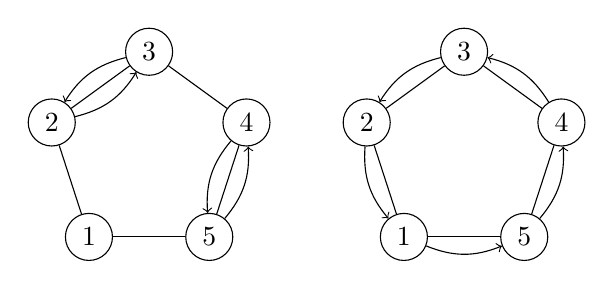
\begin{tikzpicture}
  \tikzstyle{vertex}=[draw,circle,minimum size=17pt,inner sep=0pt]

  \foreach \name/\angle/\text in {A-1/234/1, A-2/162/2, 
                                  A-3/90/3, A-4/18/4, A-5/-54/5}
    \node[vertex,xshift=5cm,yshift=.5cm] (\name) at (\angle:1.3cm) {\(\text\)};
    
 \foreach \name/\angle/\text in {B-1/234/1, B-2/162/2, 
                                  B-3/90/3, B-4/18/4, B-5/-54/5}
    \node[vertex,xshift=9cm,yshift=.5cm] (\name) at (\angle:1.3cm) {\(\text\)};

  \foreach \from/\to in {1/2,2/3,3/4,4/5,5/1}
    \draw (A-\from) -- (A-\to);
\draw[->] (A-5) to [out=50,in=-86] (A-4);
\draw[->] (A-4) to [out=-130,in=94] (A-5);
\draw[->] (A-3) to [out=194,in=58] (A-2);
\draw[->] (A-2) to [out=14,in=238] (A-3);

  \foreach \from/\to in {1/2,2/3,3/4,4/5,5/1}
    \draw (B-\from) -- (B-\to);
\foreach \to/\from in {1/2,2/3,3/4,4/5,5/1}
\draw[->] (B-\from) to [out={50 - \from * 72},in={- 86 - \from * 72}] (B-\to);
\end{tikzpicture}
\caption{An easy example for the two kinds of permutations of a chordless simple cycle that maps vertices to neighbors.}
\end{figure}
Lets assume it is mapped to \(j\in S\), then \(j\) has again two possible images under \(\sigma\) namely \(i\) and a second vertex \(k\in\mathcal Y\). If \(j\mapsto i\), no other vertex can be mapped to \(i\) or \(j\), however some other items can be swapped in the same way. The permutations of this form correspond exactly to the pairings of \(S\) and are represented in the first sum in \eqref{pmcl}. If however \(j\) is not mapped back to \(i\) but rather to its other neighbor \(k\), then \(k\) can�t get mapped back to \(j\) since \(\sigma\) is injective. Thus it has to be mapped to its other neighbor \(l\in\mathcal Y\). Through a repetition of this argument shows that this induces until \(i\) is reached again. Since the cycle is simple this path exhausts the entire cycle. The factor \(2\) is due to the fact that this shift of the indices can be done into either direction.
%A repetition of this argument shows that this chain of mappings has to continue until \(i\) is reached again. Since the cycle is chordless 
\end{proof}

\begin{prop}[Sign determines principals minors]
The knowledge of all principal minors up to size two and the sign function
\[\operatorname{sgn}\colon\mathcal C\to\left\{ \pm1\right\}\]
completely determines all principal minors of \(K\).
\end{prop}
\begin{proof}
Let \(S\subseteq\left\{ 1, \dots, N\right\}\) be arbitrary. We will again work with the expression \eqref{pmcl} of the principle minor \(\Delta_S\) and fix one permutation \(\sigma\). We can assume without loss of generality that \(\left\{ i, \sigma(i)\right\}\in E_K\) because the product it trivial otherwise. Since we know the absolute values of the off diagonal elements and the diagonal elements from the principle minors up to size two, it suffices to express the sign
\begin{equation}\label{e3.2}
\prod_{i\in S} \operatorname{sgn}(K_{i\sigma(i)})
\end{equation}
of the product through the sign function. For this we %fix one permutation \(\sigma\) and 
write \(\sigma\) as the product of disjoint cycles
\begin{equation}\label{e3.3}
\sigma = \sigma_1\circ \dots \circ \sigma_m
\end{equation}
where \(\sigma_k\colon D_k\to D_k\) for \(k = 1, \dots, m\) and the domains \(D_k\) are pairwise disjoint. The sign \eqref{e3.2} can be written as the product of
\[\prod_{i\in D_k} \operatorname{sgn}(K_{i\sigma_k(i)})\]
so it suffices to give expressions for those. Note that we could assume \(\left\{ i, \sigma_k(i)\right\}\in E_K\) and therefore \(C_k = (D_k, E_k)\) with
\[E_k = \left\{ \left\{ i, \sigma_k(i)\right\} \mid i\in D_k\right\}\]
is a cycle and therefore \eqref{e3.3} is equal to \(\operatorname{sgn}(C_k)\).
\end{proof}

\begin{theo}%[�]
Let \(K\in\mathbb R^{N\times N}\) be a symmetric matrix and \(l\) be the sparsity of its adjacency graph. Then the principal minors up to size \(l\) uniquely determine all principal minors of \(K\) and therefore the matrix \(K\) up to determinantal equivalence.
\end{theo}
\begin{proof}
In the light of the previous proposition it suffices to show that the sign function is uniquely specified by the principle minors up to size \(l\). Recall that the sign function is determined by its values on a shortest maximal cycle basis, which consists by definition of simple chordless cycles of length at most \(l\). However under the knowledge of the diagonal elements and the absolute values of the off diagonal ones, the sign of those simple chordless cycle is uniquely determined by the principle minors up to size \(l\) using the euqality \eqref{pmcl} .
\end{proof}
%\begin{rem}
%One can even show that this result is optimal in the sense that if one only has access to the principle minors up to size \(l-1\), then the equivalence class is not uniquely determined. See \cite{urschel2017learning} for details on this.\todo{can one also see this optimality from my proof?} \todo{comment on algorithms}
%\end{rem}
\begin{rem}
One can even show that this result is optimal in the sense that if one only has access to the principle minors up to size \(l-1\), then the equivalence class is not uniquely determined. To see this, we note that the sign function is not uniquely specified through the principle minors up to size \(l-1\) and thus there is more than one extension of the sign function onto the shortest maximal cycle basis. The equation \eqref{pmcl} shows that those different extensions give rise to different principle minors.
%See \cite{urschel2017learning} for details on this.\todo{can one also see this optimality from my proof?} \todo{comment on algorithms}
\end{rem}

\begin{emp}[Construction of the equivalence class]\label{cec}
We have shown that the determinantal equivalence class of a symmetric matrix is uniquely specified by its principle minors up to size \(l\). Now we want to investigate how this equivalence class can be computed and we will see that we can reduce this task to the solution of a system of linear equations over the finite field \(\mathbb F_2\).

Let us assume that we have knowledge of the principle minors \(\Delta_S\) for every \(S\subseteq\left\{ 1, \dots, N\right\}\) with size at most \(l\) and we want to construct a matrix \(\tilde K\) that is determinantally equivalent to \(K\). We have seen that we only need to reconstruct the signs of the off diagonal entries of \(K\) which is equivalent to reconstructing the edge weight \(w_{ij}\). To do this fix a shortest maximal cycle basis \(\left\{ C_1, \dots, C_m\right\}\) with vertex sets \(S_1, \dots, S_m\). Let us now rewrite \eqref{pmcl} in the form
\[H_k\coloneqq \Delta_{C_k} - \!\! \sum_{P\in\mathcal P(C_k)} (-1)^{\left\lvert P \right\rvert}\cdot \!\!\!\prod_{\left\{ i, j\right\}\in P}\! K_{ij}^2 \cdot\!\!\prod_{i\notin V(P)}\! K_{ii} = 2 \cdot (-1)^{\left\lvert C_k \right\rvert + 1} \operatorname{sgn}(C_k)\cdot\!\!\!\! \prod_{\left\{ i, j\right\}\in C_k}\left\lvert K_{ij} \right\rvert. \]
Given the principle minors, we can determine the value on the right side and taking the sign on both sides yields
\[ (-1)^{\left\lvert C_k \right\rvert + 1} \cdot \operatorname{sgn}(H_k) = \operatorname{sgn}(C_k) = \prod_{\left\{ i, j\right\}\in E(S_k)} w_{ij} \]
which we seek to solve for \(w\). However this multiplicative equation is hard to solve and therefore we use the canonical group isomorphism \(\phi\) between \(\left\{ \pm 1\right\}\) and \(\left\{ 0, 1\right\}\) to turn it into a linear equation. Setting \(x_{ij}\coloneqq \phi(w_{ij})\) we get that the condition above is equivalent to
\begin{equation*}
b_k\coloneqq \phi( \operatorname{sgn}(H_k)) + \lvert \hat S_k \rvert + 1 = \sum_{\left\{ i, j\right\}\in E(S_k)} x_{ij} = (Ax)_k \quad \text{in } \mathbb F_2
\end{equation*}
where \(A\) is the matrix with the rows \(x(C_k)^T\). Now we can fix any such solution \(x %= \phi(w)
\in\mathbb F_2^{E}\) of
\begin{equation}\label{linEqu}
Ax = b
\end{equation}
and we know that at least one exists, namely the one given by \(x_{ij} = \phi(\operatorname{sgn}(K_{ij}))\). %In the light of \eqref{e3.0} i
Let now \(w_{ij}\coloneqq x_{ij}\), then it is straight forward to see that \(\tilde K\) defined through
\[\tilde K_{ii} \coloneq\Delta_{\left\{ i\right\}} \quad\text{and } \tilde K_{ij} = w_{ij} \cdot \sqrt{\tilde K_{ii}\tilde K_{jj} - \Delta_{\left\{ i, j\right\}}} \]
is determinantally equivalent to \(K\).
%More precisely we seek to find weight \(w_{ij}\) such that \eqref{pmcl} holds. This is the case if and only if
\end{emp}

It shall be noted that there are algorithms with much better computational performance for the construction of the determinantal equivalence class. For some examples of efficient algorithms we refer to \cite{urschel2017learning} and \cite{rising2015efficient}.

%This is known as the \emph{principal minor assignment problem} and has been studied extensively (cf. \cite{griffin2006principal} and \cite{urschel2017learning}) and an computationally efficient algorithm has been proposed for the problem in \cite{rising2015efficient}. It is in fact possible to retain the matrix from its principal minors up to an equivalence relation which identifies matrices with each other, that have the same principal minors. Obviously this is sufficent for the task of learning a DPP, because those matrices are exactly those who give rise to the same point process. To see roughly how this reconstruction works we note that the diagonal is given by
%\[K_{ii} = \det(K_{\left\{ i\right\}})\]
%and the absolute value of the off diagonal can be obtained through
%\[K_{ij}^2 = K_{ii} K_{ii} - \det\big(K_{\left\{ i,j\right\}}\big). \]
%The reconstruction of the signs of the entries \(K_{ij}\) turns out to be the main difficulty, but this can be done analysing the cycles of the adjacency graph \(G_K\) corresponding to \(K\).%\todo{see whether this proof can be done in a simplified way without considering the sparsity \(l\)}
% The adjacency graph has \(\mathcal Y\) as its vertex set and the set of edges consists of the pairs \(\left\{ i,j\right\}\) such that \(K_{ij}\ne0\). The reconstruction now relies on the analysis of the cycles of this graph and it has been shown, that one only needs to know all the principal minors up to the order of the cycle sparsity of \(G_K\) (cf. \cite{urschel2017learning}). Following this method it is possible to compute estimators \(\hat K_n\) of \(K\) in polynomial time and give a bound on the speed of convergence in some suitable metric.\todo{state and assymptotic the result}

% In completely analogue fashion one can learn the elementary kernel \(L\).
% and those estimations can be used to sample from a DPP that was observed. This procedure might be sufficient in some scenarios, but this approach lacks the ability to extrapolate the knowledge one has of specific DPPs onto some new, unobserved DPPs which is exactly the point that would distinguish the procedure from classical statistics and would allow for far more interesting applications. To achieve this, we introduce the notion of conditional DPPs in the following section which are customised to describe families of DPPs with kernels that are in some way similar.#

%\subsubsection*{Definition of the estimator}


So far we have seen that the principle minors determine a symmetric matrix up to determinantal equivalence. However the empirical marginal densities do not in general need to be the principle minors of any symmetric matrix, in other words the empirical measures are not necessarily determinantal. Therefore the definition of the estimator is till not quite straight forward and we will follow \cite{urschel2017learning} for this and make the following assumption.

\begin{emp}[Assumption]\label{ass}
Let \(\alpha>0\) and assume that 
\[\min\left\{ \left\lvert K_{ij} \right\rvert\mid K_{ij}\ne0\right\}\ge\alpha.\]
\end{emp}

Note that such an \(\alpha\) can always be found, however it is not a priori known. For example if we want to make a statement about the speed of approximation of the estimators , which depends on \(\alpha\), we have to make the assumption above.

%An important quantity in the estimation of the kernel \(K\) is
%\[\alpha\coloneqq\min\left\{ \left\lvert K_{ij} \right\rvert\mid K_{ij}\ne0\right\}>0. \]
%Note that this quantity is not a priori known.

\begin{emp}[Definition of the estimator]\label{DefEst}
The straight forward estimators of the principal minors are
\[\hat\Delta_S \coloneqq \hat{\mathbb P}_n(S\subseteq\mathbf Y) \quad \text{for }S\subseteq\left\{ 1, \dots, N\right\}. \]
The resulting estimates for the diagnoal elements and the squares of the off diagonals are
\[\hat K_{ii} \coloneqq \hat\Delta_{\left\{ i\right\}} \quad \text{and } \hat B_{ij}\coloneqq \hat K_{ii}\hat K_{jj} - \hat\Delta_{\left\{ i, j\right\}}.\]

Next we will introduce an estimate \(\hat G\) for the adjacency graph and will then try to choose the signs of the estimated matrix \(\hat K\) such that the its principal minors are the estimates for the principal minors. For this define the edge set \(\hat E\) of \(\hat G\) to consist of all sets \(\left\{ i, j\right\}\) such that \(\hat B_{ij}\ge\frac12\alpha^2\). This truncation yields the desired effect that by the strong law of large numbers the estimator for the graph will converge to the actual adjacency graph almost surely. In analogy to the previous paragraph we define \(\{ \hat C_1, \dots, \hat C_{\hat m}\}, \hat H_1, \dots, \hat H_{\hat m}, \hat A\) and \(\hat b\) exactly the same way. If there is a solution \(\hat x\in\mathbb F_2^{E}\) to the linear equation
\begin{equation}\label{LinEqu2}
\hat A\hat x = \hat b,
\end{equation}
then we estimate the signs to be \(\hat w_{ij}\coloneqq \phi^{-1}(\hat x_{ij})\) and define \[\hat K_{ij} \coloneqq \hat w_{ij} \sqrt{\hat B_{ij}}.\]

%If the procedure described in \ref{cec} works, namely if \eqref{linEqu} posseses a solution, then we will define our estimator \(\hat K\) this way.
If there is no such solution \(\hat x\) then we simply set the signs of the off diagonal elements to be positive, i.e. we define \[\hat K_{ij}\coloneqq \sqrt{\hat B_{ij}}.\] This choice is completely arbitrary, but we will see in the consistency result \ref{MomCon} that the probability for this case tends to zero as the sample size increases. In fact we will see that the two linear equations \eqref{linEqu} and \ref{LinEqu2} agree with increasing probability.
\end{emp}

%This means that every edge \(\left\{ i, j\right\}\in E\) will be contained in each estimator for large sample size and 

%Let further \(\left\{ \hat C_1, \dots, \hat C_k\right\}\) be a shortest maximal cycle basis where \(\hat S_l\) is the set of vertices of \(\hat C_l\). Define now
%\[\hat H_k\coloneqq \hat \Delta_{\hat S_l} - \sum_{P\in\mathcal P(\hat S_l)} (-1)^{\left\lvert P \right\rvert} \prod_{\left\{ i,j\right\}\in P}\hat B_{ij} \prod_{i\notin V(P)} \hat K_{ii}. \]
%In the light of \eqref{pmcl} we wish to choose the signs \(\hat w_{ij}\) of \(\hat K_{ij}\) in such a way that the resulting signs of the cycles \(\hat C_l\) satisfy
%\[\operatorname{sgn}(\hat H_l) \cdot(-1)^{\lvert \hat S_l \rvert + 1} = \operatorname{sgn}(\hat C_l) = \prod_{\left\{ i, j\right\}\in E(\hat S_l)}\hat w_{ij}.\]
%To turn this product equation in \(\hat w\) into a linear equation we use the canonical group isomorphism \(\phi\) between \(\left\{ \pm 1\right\}\) and \(\left\{ 0, 1\right\}\). Setting \(\hat x_{ij}\coloneqq \phi(\hat w_{ij})\) we get that the condition above is equivalent to
%\[b_l\coloneqq \phi( \operatorname{sgn}(\hat H_l)) + \lvert \hat S_l \rvert + 1 = \sum_{\left\{ i, j\right\}\in E(\hat S_l)} \hat x_{ij} = (A\hat x)_l\]
%where \(A%\in\mathbb F_2^{k\times E}
%\) is the matrix with the rows \(x(\hat C_l)^T\). Either such a solution \(\hat x = \phi(\hat w)\in\mathbb F_2^{E}\) exists or we set \(\hat w\coloneqq (1, \dots, 1)^T\). Finally we define the estimator via
%\[\hat K_{ij}\coloneqq \begin{cases}  \hat w_{ij}\cdot \sqrt{(\hat B_{ij})} \quad & \text{if } \left\{ i, j\right\}\in \hat E \\ 0 & \text{if } \left\{ i, j\right\}\notin \hat E \end{cases}. \]
 %and otherwise
% \[\hat K_{ij}\coloneqq \sqrt{(\hat B_{ij})}.\]

In order to talk about consistency of the estimator that we constructed above, it is necessary to define a metric on the marginal kernels of DPPs. However the usual operator norm is clearly not right for this job, since we already know that we can only hope to reconstruct the determinantal equivalence class but not the exact marginal kernel. Thus we will work with the usual choice of pseudometric if one has to deal with equivalence classes.

\begin{emp}[Pseudometric on the marginal kernels]
We define the distance between two marginal kernels \(A, B\in\mathbb R^{N\times N}\) through
\[d(A, B)\coloneqq \inf_{C\sim A}\left\lVert B - C \right\rVert_\infty \]
where \(\left\lVert A \right\rVert_\infty\coloneqq \max_{1\le i, j\le N} \left\lvert A_{ij} \right\rvert\) denotes the uniform norm on the space of matrices.
\end{emp}

\begin{theo}[Consistency]\label{MomCon}
Let \(K\) be the marginal kernel of a DPP that satisfy the assumption \ref{ass}. Let further \(l\) be the cycle sparsity of \(G_K\) and \(\varepsilon>0\). 
%Then for any \(A>0\) there is a constant \(c>0\) such that for every
%\[n\ge c\cdot\left( \frac{\varepsilon^2}{\alpha^2} + l\cdot\left( \frac{4}{\alpha}\right)^{2l}\right) \cdot \log(N)\]
%we have \(d(\hat K, K)\le\varepsilon\) with probability at least \(1 - N^{-A}\).
\[\mathbb P\left(d(\hat K, K)\ge\varepsilon\right) \to 0\quad\text{for } n\to\infty. \]
\end{theo}
\begin{proof}
We will keep the notations from the paragraphs \ref{cec} and \ref{DefEst}.
%We will prove that the probability that \ref{linEqu} and \eqref{LinEqu2} agree tends to one. 
%We refer to \cite{urschel2017learning}.
We have already seen in the motivation of this section that the empirical measures converge almost surely which directly implies
\begin{equation}\label{asc}
%\hat\Delta_S\to\Delta_S 
\hat K_{ii}\to K_{ii}\quad\text{and } \hat K_{ij}^2 \to K_{ij}^2 \quad \text{almost surely}.
\end{equation}
Note that almost surely convergence implies convergence in probability and thus we have
\[\mathbb P(\hat G = G_K) = \mathbb P\left(\hat K_{ij}^2 \ge \alpha^2/2 \text{ for } K_{ij}\ne0\right) \to 1 \quad\text{for } n\to\infty.\]
In this case the two shortest cycle basis can be chosen the same and so \(\hat A\) and \(A\) agree. %Hence we have
%\begin{equation*}%\label{ConProb1}
%\mathbb P(\hat A = A)\to 1 \quad\text{for } n\to\infty.
%\end{equation*}
Because of \eqref{asc} we also have \(\hat H_k\to H_k\) almost surely and thus \(\hat b_k\to b_k\) almost surely for all \(k\). This yields
\begin{equation}\label{ConProb1}
\mathbb P\left(\hat A = A \text{ and } \hat b = b\right)\to 1 \quad\text{for } n\to\infty.
\end{equation}
In this case the two linear quations \eqref{linEqu} and \eqref{LinEqu2} agree, then \(\tilde K\in\mathbb R^{N\times N}\) defined through \(\tilde K_{ij}\coloneqq \hat w_{ij}\left\lvert K_{ij} \right\rvert\) is determinantally equivalent to \(K\). Further we know that for any \(\delta>0\)
\begin{equation}\label{ConProb2}
\mathbb P\left(\left\lvert \hat K_{ij}^2 - K_{ij}^2 \right\rvert < \delta \text{ for all } i, j \right)\to1 \quad \text{for } n\to\infty.
\end{equation}
If this is true, then we have
\[d(\hat K, K) \le \lVert \hat K - \tilde K \rVert_{\infty} = \sup_{i, j} \left\lvert \lvert \hat K_{ij} \rvert- \lvert \tilde K_{ij} \rvert \right\rvert \]
where we used, that the entries of \(\hat K\) and \(\tilde K\) have equal signs. Further we have %\(\lvert \hat K_{ii} - \tilde K_{ii} \rvert < \delta\) as well as
\[\left\lvert \lvert \hat K_{ij} \rvert- \lvert \tilde K_{ij} \rvert \right\rvert = \frac{\big\lvert \hat K_{ij}^2 - \tilde K_{ij}^2 \big\rvert}{\lvert \hat K_{ij} \rvert + \lvert \tilde K_{ij} \rvert} < \frac{\delta}{\alpha}\le\varepsilon \]
if \(\delta \le \alpha\varepsilon\). In conclusion we have seen that if
\[\hat A = A, \quad \hat b = b \quad\text{and } \left\lvert \hat K_{ij}^2 - K_{ij}^2 \right\rvert < \delta \quad \text{for all } i, j\]
then we have
\[d(\hat K, K) < \varepsilon.\]
However \eqref{ConProb1} and \eqref{ConProb2} shows that the probability for this tends to one.
%Let now \(\left\{ C_1, \dots, C_m\right\}\) be a maximal shortest cycle basis of \(G_k\) with corresponding vertex sets \(S_1, \dots, S_m\). Let further 
%\[H_k\coloneqq2\cdot\!\!\!\!\!\!\prod_{\left\{ i, j\right\}\in E(S_k)}\!\!\!\!\!\! K_{ij} \quad \text{and } \hat H_k\coloneqq2\cdot\!\!\!\!\!\!\prod_{\left\{ i, j\right\}\in E(S_k)}\!\!\!\!\!\! \hat K_{ij}.\]
%\(H_k\) be like in \ref{cec} and \(H_{}
%Now \eqref{asc} implies
%\[\hat H_k\to H_k \quad \text{almost surely}.\]
%In particual those convergences hold in probability and therefore we have
%\[\mathbb P\left( \left\lvert \hat H_k- H_k \right\rvert\le\delta \text{ or } \left\lvert \hat K_{ii} - K_{ii} \right\rvert \le \delta \text{ or } \left\lvert \hat K_{ij}^2 - K_{ij}^2 \right\rvert \le \delta \text{ for all } k, i, j \right)\to0 \quad \text{for } n\to\infty.\]
%Hence it suffices to show that
%\[\left\lvert \hat H_k - H_k \right\rvert < \delta, \left\lvert \hat K_{ii} - K_{ii} \right\rvert < \delta \quad \text{and } \left\lvert \hat K_{ij}^2 - K_{ij}^2 \right\rvert < \delta \]
%for all according \(k, i, j\) implies \(d(\hat K, K)<\varepsilon\) where \(\delta\) is still to be determined. 
\end{proof}

\begin{rem}[Speed of convergence]
Although the result above states that the estimators \(\hat K\) converges to \(K\) in probability, it does give no information about the speed of convergence. This problem is addressed in \cite{urschel2017learning}, but it turns out that the convergence is very slow. For example for the very moderate case \(\alpha = 0.4\) and \(l=3\) one already needs more than \(10^6\) samples to get some theoretical guarantees from their result. This is not due to careless estimates since they even show that this bound is optimal\todo{is this true?}. However since this result is beyond practical relevance, we will keep away from those calculations.
\end{rem}
\todo{explain how the algorithm for the reconstruction works}
%\todo{how hard it is to prove}
\todo{is this estimator unbiased?}

\section{Maximum likelihood estimation using optimisation techniques}

The method of maximum likelihood estimation is a very well established procedure to estimate parameters. The philosophy of MLE is that one selects the parameter under which the given data would be the most likely to be observed and to motivate this in more detail we roughly follow the corresponding section in \cite{rice2006mathematical}.
%Assume again that we have \(n\) samples \(\mathbf Y_1, \dots, \mathbf Y_n\) and then the maximum likelihood estimator would be the kernel 

For example we might consider a sequence random variables \(X_1, \dots, X_n\) with a joint density \(f(x_1, \dots, x_n, \theta)\) with respect to some reference measure \(\prod_{i=1}^n\mu(\mathrm d x_i)\). Now we want to estimate the parameter \(\theta\) based on a sample \(x_1, \dots, x_n\) of our random variables. Then one reasonable guess for \(\theta\) would be the one under which the observation of those observations \(x_1, \dots, x_n\) is the most likely. In other words we want to find the parameter \(\theta\) that maximises the density \(f(x_1, \dots, x_n, \theta)\). If additionally the random variables are indepent and identically distributed, their joint density factorises and thus we obtain
\[f(x_1, \dots, x_n, \theta) = \prod_{i=1}^n f(x_i, \theta) \]
where \(f(x, \theta)\) is the density with respect to \(\mu\) of the \(X_i\). In practice it is often easier to maximise the logarithm of the density
\[\mathcal L(\theta) = \log\!\big(f(x_1, \dots, x_n, \theta)\big) = \sum_{i=1}^n \log\!\big(f(x_i, \theta)\big) \]
 since this transforms the product over functions into a sum. However this is clearly equivalent to maximising the density since the logarithm is strictly monotone. We call the function \(\mathcal L\) the \emph{log likelihood function} and we denote its domain which is just the set of all parameters we wish to consider by \(\Theta\). Further we call its maximiser
 \[\hat \theta_n\coloneqq \underset{\theta\in\Theta}{\arg\max} \mathcal L(\theta) \]
the \emph{maximum likelihood estimater} or short MLE.

% \todo{general blabla about MLE}

\todo{Reminder on optimisation}



\subsection{Presentation of different models}

Assume again that we have a set of observations \(Y_1, \dots, Y_n\subseteq\mathcal Y\) drawn independently and according to the DPP \(\mathbb P\). This time we want to find the maximum likelihood estimator for the elementary kernel and in order to do this we need to be able to express the density of the DPP which is nothing but the values of the elementary probabilities. Thus we will assume that we are dealing with \(L\)-ensembles in this section. We will present the maximum likelihood estimators for different parametric classes of DPPs.

\subsubsection*{MLE of the elementary kernel \(L\)}

The most intuitive parameter that one can estimate is the elementary kernel \(L\) itself since it parametrises the entire class of \(L\)-ensembles.

\begin{emp}[Maximum likelihood estimator for \(L\)]
We seek to find the MLE 
\[\hat L_n \coloneqq \underset{L\in\mathbb R^{N\times N}_{\text{sym}, +}}{\arg\max}\, \mathcal L(L) \]
for the elementary kernel \(L\) in the set \(\mathbb R^{N\times N}_{\text{sym}, +}\) of all symmetric and positive semidefinite \(N\times N\) matrices. The log likelihood function is now given by
%We aim to establish a quantity that gives an intuitive measure of how well a different DPP describes the training set and then we want to find the elementary kernel \(L\) for which the associated DPP \(\mathbb P_L\) optimises this quantity. A widely used choice in the machine learning community for this is the so called \emph{log likelihood function}
\[\mathcal L \colon\mathbb R^{N\times N}_{\text{sym}, +} \to [-\infty, 0], \qquad L \mapsto \log\left(\prod_{i = 1}^n \mathbb P_L(Y_i)\right).\]
\end{emp}
Using \eqref{e2.3} we get the expression
\begin{equation}\label{e3.1}
\mathcal L(L) = \sum\limits_{i=1}^n\log\left( \det(L_{Y_i})\right) - n \log\left( \det(L+I)\right).
\end{equation}
Although the parametric family of that arises from the elementary kernels \(L\) gives a high variety of different associated \(L\)-ensembles, it will also make the computation of the MLE more complex. Therefore we will consider some smaller classes of \(L\)-ensembles, which will decrease the flexibility of the model, but make computation more efficient.

\subsubsection*{MLE of the qualities}

Unlike earlier we will not try to estimate the whole kernel \(L\) but only the qualities \(q_i\) of the items \(i\in\mathcal Y\). More precisely we recall that we can parametrise the positive definite symmetric matrices \(L\) using the quality diversity parametrisation %decomposition %, i.e. we consider the bijection\todo{whats the domain?}
\[ (q, S) \mapsto \Psi(q, S) = L \quad \text{where } L_{ij} = q_iS_{ij}q_j.\]
Now we fix a similarity kernel \(\hat S\), that we will usually model according to some perceptions we might have, and will only try to estimate the quality \(q\in\mathbb R_+^N\). This means that we optimise the likelihood function over a smaller set of kernels, namely the ones of the form \(\Psi(q, \hat S)\) for \(q\in\mathbb R_+^N\). Obviously the maximal likelihood that can be achieved using this more restrictive model decreases since we consider less positive definite matrices and we have %will be lower compared to the one obtained by a full kernel estimation, since we have
\[\max_{q\in \mathbb R_+^N} \mathcal L(\Psi(q, \hat S)) \le %\max_{(q, S)\in \mathbb R_+^N\times \mathbb S_N^N} \mathcal L(\Psi(q, S)) =
 \max_{L\in \mathbb R_{\text{sym}, +}^{N\times N}} \mathcal L(L). \]\todo{sort out notation problem with \(S\) and \(\phi\)}
 \todo{sort out notation problem with \(N\) and \(\mathcal Y\)}
 
Although we can only expect a worse descriptive power of the observation, the hope is that the task of estimating only the qualities \(q\in\mathbb R_+^N\) is more feasible which actually turn out to be true in certain cases. But before we investigate this, we clearly state our goal.

\begin{emp}[Maximum likelihood estimator for the quality]
% {\scshape\bfseries .}
 We aim to find the MLE of the quality vector \(q\in\mathbb R_+^N\), in other words we are interested in the existence and the computability of the quantity
\[\hat q_n \coloneqq \underset{q\in\mathbb R_+^N}{\arg\max}\, \mathcal L(\Psi(q, \hat S)) \]
where the likelihood is still given by \eqref{e3.1}.
\end{emp}

Since we are only interested in estimating the quality vector \(q\in\mathbb R_+^N\), we will perceive the log likelihood function as a function of \(q\). Further we notice that the single summands take the form following form\todo{refer to the equation!}
\begin{equation}\label{loglikqua}
% \mathcal L(\Psi(q, \hat S)) & = \sum\limits_{i = 1}^n 
\log\left( \prod_{j\in Y_i} q_j^2\right) + \log(\det(\hat S_{Y_i})) - \log\left(\sum_{A\subseteq \mathcal Y} \prod_{j\in A}q_j^2\det(\hat S_A) \right).
% \\ & = \sum\limits_{i = 1}^n \log\left( \prod_{j\in Y_i} q_j^2\right) \cdot \det(\hat S_{Y_i}) - n
\end{equation}

\subsubsection*{Log linear model for the qualities}

The motivation for restricting our ambitions of estimation to the qualities \(q_i\) rather than the whole elementary kernel \(L\in\mathbb R_{\text{sym}, +}^{N\times N}\) was to obtain a more tractable optimisation problem. 
%In order to see whether we succeeded in that regard, we note that each summand in the log likelihood function takes the following form under the quality diversity parametrisation
%perceive -- without change of notation -- the log likelihood function now as a function of the quality vector, i.e. \(\mathcal L\colon \mathbb R_+^N\to [-\infty, 0]\) where
%\begin{equation}
% \mathcal L(\Psi(q, \hat S)) & = \sum\limits_{i = 1}^n 
%\log\left( \prod_{j\in Y_i} q_j^2\right) + \log(\det(\hat S_{Y_i})) - \log\left(\sum_{A\subseteq \mathcal Y} \prod_{j\in A}q_j^2\det(\hat S_A) \right).
% \\ & = \sum\limits_{i = 1}^n \log\left( \prod_{j\in Y_i} q_j^2\right) \cdot \det(\hat S_{Y_i}) - n
%\end{equation}
Unfortunately we can tell from \eqref{loglikqua} that the log likelihood still isn�t concave in \(q\) and in order to achieve this, we will have to make following assumption and keep them in throughout this section.\todo{does it makes sense?}

%{\scshape\bfseries .}
\begin{emp}[Log linear model for the qualities]
From now on we will fix vectors \(f_i\in\mathbb R^M\) for \(i\in\mathcal Y\) and call them \emph{feature vectors}. Further we set
\[q_i = \exp\left(\frac12 \theta^T f_i\right)\quad \text{for } \theta\in\mathbb R^M\]
and will only consider quality vectors \(q\in\mathbb R_+^N\) that have this form.
\end{emp}

\begin{rem}
It shall be noted that although this log linear model seems to be a harsh restriction, it isn�t a restriction at all, at least theoretically. If we take \(M=N\) and choose \(f_i\) to be the unit vectors in \(\mathbb R^N\), then this just a logarithmic transformation of the parameters and thus the maximal likelihood that can be achieved with this model does not change. In practice however it will be of interest to work with rather low dimensional parameters \(\theta\), because if the ground set \(\mathcal Y\) gets large, optimisation in \(\mathcal R^N\) can be inefficient. In this case of course the maximal likelihood under the optimal parameter may decrease. However the approximation of the optimal parameter might become possible again which justifies this sacrifice.
\end{rem}

Under the assumption of a log linear model for the qualities the individual terms of the log likelihood function take the form
\begin{equation}\label{e3.31}
\theta^Tf_{Y}(X) + \det(S_{Y}(X)) - \log\left( \sum_{A\subseteq\mathcal Y(X)} \exp\left( \theta^Tf_{A}(X)\right)\det(S_A(X)) \right).
\end{equation}

\subsubsection*{MLE of the repulsiveness parameter}

\subsection{Existence of the maximum likelihood estimators}

A priori it is not clear that the maximum likelihood estimators exist and we will actually see that they do not exist in general. However one can still save this approach because the probability that they exist tends to \(1\) if the sample size increases. We begin by showing this for the MLE of the qualities and then we will adapt this proof to the other models.

\subsubsection*{MLE of the qualities}

To see that the MLE \(\hat q_n\) does not exist in general, we suppose that we have only one sample \(Y_1 = \mathcal Y\) which is the whole set. The higher the qualities of the items are, the more likely this observation gets and therefore the maximum of the log likelihood function -- which is \(0\) in this case -- is not obtained. This can also be made rigorous in the following computation. Under the assumption of constant qualities the log likelihood function takes the form
\begin{equation*}
\begin{split}
\log(q^{2N} \det(\hat S_{\mathcal Y})) - \log\left(\sum_{A\subseteq \mathcal Y}q^{2\left\lvert A \right\rvert}\det(\hat S_A) \right) = \log\left( \frac{q^{2N} \det(\hat S_{\mathcal Y})}{\sum_{A\subseteq \mathcal Y}q^{2\left\lvert A \right\rvert}\det(\hat S_A)}\right) \xlongrightarrow{q\to\infty} 0.
\end{split}
\end{equation*}
However this maximum is never attained, since for every \(L\)-ensemble we have \(\mathbb P_L(\varnothing) > 0\) and therefore
\[\mathcal L(q) = \log\left(\mathbb P_{\Psi(q, \hat S)}(\mathcal Y)\right) < 0 \quad \text{for every } q\in\mathbb R_+^N. \]

The thing that goes wrong in this case is, that under the observation of the whole set \(\mathcal Y\) we would estimate a deterministic model that always selects the whole set, namely the DPP with marginal kernel \(I\). Since all of the eigenvalues are \(1\) in this case, this DPP is not a \(L\) ensemble and therefore we can not describe it with the quality diversity decomposition.
However if we assume that the data is actually generated by a \(L\)-ensemble, then such a scenario becomes unlikely as the sample size increases. We will fix this in the following result.

\begin{prop}[Existence of the MLE]
Let \(\mathbf Y_1, \mathbf Y_2, \dots\) be a sequence of independent and identically distributed point processes that fall in the class of \(L\)-ensembles. Then we have
\[\mathbb P\left(\hat q_n\in\mathbb R_+^N \text{ exists}\right) \xlongrightarrow{n\to\infty} 1.\]
\end{prop}
\begin{proof}
We will show that the MLE exists if one of the observations is the emptyset. Then the claim follows from
\begin{equation*}
\begin{split}
\mathbb P\left(\hat q_n\in\mathbb R_+^N \text{ exists}\right) & \ge \mathbb P\left(\bigcup_{i=1}^n \left\{ \mathbf Y_i = \varnothing\right\}\right) = 1 - \mathbb P\left(\bigcap_{i=1}^n \left\{ \mathbf Y_i \ne\varnothing\right\}\right) \\ 
& = 1 - \mathbb P(\mathbf Y_1 \ne\varnothing)^n \xlongrightarrow{n\to\infty} 1
\end{split}�
\end{equation*}
since we have \(\mathbb P(\mathbf Y_1 \ne\varnothing) < 1\) for every \(L\)-ensemble.

To prove that the log likelihood function possesses a maximum we will prove that it is coercive in some way, i.e. that we have
\begin{equation*}\label{coe}
\mathcal L(q)\to -\infty\quad\text{for } \left\lvert q \right\rvert\to\infty.
\end{equation*}
Elementary considerations then yield the existence of a maximiser. So let \(Y_1, \dots, Y_n\) be some observations with \(Y_i=\varnothing\) for at least one \(i\in\left\{ 1, \dots, n\right\}\). Let \((q^k)_{k\in\mathbb N}\subseteq\mathbb R_+^N\) be a  sequence such that \(\lvert q^k \rvert\to \infty\). Note that it suffices to show that ever subsequence of \((q^k)\) contains a subsubsequence \((q^l)\) such that 
\[\mathcal L(q^l)\to-\infty\quad\text{for } l\to\infty.\]
Hence we fix a subsequence of \((q^k)\) which we denote by \((q^k)\) again in slightly abusive notation. Let \((q^l)\) be a subsequence of \((q^k)\) such that one coordinate diverges to infinity, i.e.
\[q_{j_0}^l\xlongrightarrow{l\to\infty} \infty\quad\text{for one } j_0\in\left\{ 1, \dots, N\right\}.\]
The \(i\)-th summand of \(\mathcal L\) takes the form
\[-\log\left( \sum_{A\subseteq\mathcal Y}\prod_{j\in A}(q^l_j)^2\det(\hat S_A)\right) \le - \log\left( (q^l_{j_0})^2\right)\xlongrightarrow{l\to\infty} -\infty\]
where we used \(\hat S_{\left\{ j_0\right\}} = 1\). Because the other summands are non positive this implies
\[\mathcal L(q^l)\xlongrightarrow{l\to\infty} -\infty\]
which we had to show.
%. Will show that if the sequence \(\big( \mathcal L(q^k)\big)_{k\in\mathbb N}\) is bounded from below, then all coordinate sequences \((q^k_j)_{k\in\mathbb N}\) are bounded for all \(j\in\left\{ 1, \dots, N\right\}\). Note that this is equivalent to \eqref{coe}.
\end{proof}

\begin{rem}
The proof above should be read in the following way. The statement \(q^l_{j_0}\to\infty\) is equivalent to a model that would always select the item \(j_0\). However since we have observed the empty set, the observations would be impossible under this model and thus the log likelihood function takes the value \(-\infty\) for this model. An analogue argument shows that the estimated qualities are strictly positive with high probability if the actual qualities are strictly positive. This will be of interest for us if we consider the log linear model.
\end{rem}

\begin{prop}[Positivity of the MLE]\label{PosMLE}
Assume that \(\mathbf Y_1, \mathbf Y_2, \dots\) is a sequence of independent and identically distributed point processes that are distributed according to a \(L\)-ensemble with strictly positive qualities. Then we have
\[\mathbb P\left(\hat q_n\in\mathbb R_+^N \text{ exists and } \hat q_n\in (0, \infty)^N\right) \xlongrightarrow{n\to\infty} 1.\]
\end{prop}
\begin{proof}
We have already seen that the probability that the MLE exists tends to one, so we only have to show that the probability that the estimated qualities are strictly positive tends to one. The philosophy to prove this is exactly the same than in the proof of existence. Indeed we note that once \(j\) occurs in one of the observations \(Y_1, \dots, Y_n\) we have \(\mathcal L(q) = -\infty\) for every \(q\in\mathbb R_+^N\) with \(q_j = 0\). Therefore we have \((\hat q_n)_j>0\) if \(j\in Y_i\) for at least one \(j\in\left\{ 1, \dots, n\right\}\). Finally we note that the probability that \(j\) occurs in the \(i\)-th sample is strictly positive since we have
\[\mathbb P(j\in\mathbf Y_i)\ge\mathbb P(\left\{ j\right\} = \mathbf Y_i) = q_j^2>0. \]
\end{proof}

\subsubsection*{MLE of the elementary kernel}

We can quite easily adapt the proof for the existence of MLEs of the qualities to the case of MLEs for the whole elementary kernel \(L\).

\begin{prop}[Existence of MLE for the kernel]
Let \(\mathbf Y_1, \mathbf Y_2, \dots\) be an sequence of independent and identically distributed point processes that fall in the class of \(L\)-ensembles. Then we have
\[\mathbb P\left(\hat L_n\in\mathbb R^{N\times N}_{\text{sym}, +} \text{ exists}\right) \xlongrightarrow{n\to\infty} 1.\]
\end{prop}
\begin{proof}
To recycle the proof above we note that it suffices to show \(\mathcal L(L)\to -\infty\) for \(\left\lvert L \right\rvert\to\infty\) once we have observed the empty set once. To see this, we use the quality diversity parametrisation
\[\Psi\colon\mathbb R_+^N\times\mathbb S_N^N\to\mathbb R^{N\times N}_{\text{sym}, +}, \quad (q, \phi)\mapsto \left( q_i\phi_i^T\phi_j q_j\right)_{1\le i, j\le N}.\]
Note that since \(\Psi\) is continuous and therefore bounded on bounded sets and \(\mathbb S_N^N\) is bounded, \(\left\lvert \Psi(q, \phi) \right\rvert\to\infty\) implies \(\left\lvert q \right\rvert\to\infty\). The exact same calculations as in the previous proof show
\[\mathcal L(L) = \mathcal L(\Psi(q, \phi))\to-\infty\quad \text{for }\left\lvert L \right\rvert\to\infty.\]
\end{proof}

\subsubsection*{The log linear model}

We have seen that the log linear model can provide a parametrisation of the whole space \((0, \infty)^N\) of possible qualities. However it can also be very ristrictive, for example if all feature vectors are trivial, i.e. \(f_i = 0\) for all items \(i\). Hence we need to convince ourselves that we do not loose too much information through the transformation %a way to determine whether the transformation
\[F\colon\mathbb R^M \to (0, \infty)^N, \quad \theta\mapsto \big(\exp(\theta^Tf_1), \dots, \exp(\theta^Tf_N)\big)^T.\]
%loses enough information for the MLE to exist.
In order to do this, let \(U\subseteq\mathbb R^M\) be the span of \(f_1, \dots, f_N\) and let write \(\theta = \theta_1 + \theta_2\) such that \(\theta_1\in U\) and \(\theta_2\in U^\perp\). We note that \(F(\theta) = F(\tilde\theta)\) if and only if \(\theta_1 = \tilde\theta_1\).

\todo{show that coercivity and identifiability is the same!}
%\begin{emp}[Coercivity of the log linear model]
%We call the log linear model \emph{coercive}, if whenever we have \(\left\lvert \theta_k \right\rvert\to\infty\) there is at least one index \(i\in\left\{ 1, \dots, n\right\}\) and one subsequence \((q_l)\) of \((q_k)\) such that
%we have
%\[\exp(\theta_l^Tf_i) \to \infty \quad \text{or } \exp(\theta_l^Tf_i) \to 0 \quad \text{for } l\to\infty. \]
%whenever \(\left\lvert \theta_ \right\rvert\)
%\end{emp}

%In the proof of following result we see how the coercivity is exactly the property that allows us to adapt the prove of existence of the MLE we have used before.

\begin{prop}[Existence of MLE]
Assume that \(\mathbf Y_1, \mathbf Y_2, \dots\) is a sequence of independent and identically distributed point processes that are distributed according to a \(L\)-ensemble with strictly positive qualities. Then we have
\[\mathbb P\left(\hat \theta_n\in\mathbb R^M \text{ exists}\right) \xlongrightarrow{n\to\infty} 1.\]
\end{prop}
\begin{proof}
First we note, that it suffices to show that \(\mathcal L\) has a maximiser on \(U\), since \(F(U) = F(\mathbb R^M)\). To do this we show -- just like in the previous cases -- that the \(\mathcal L\) is coercive on \(U\) whenever we have observed the emptyset as well as every item at least once. Let now \((\theta^k)_{k\in\mathbb N}\subseteq U\) be a sequence such that \(\lvert \theta^k \rvert\to\infty\). Then there is at least one index \(i\in\left\{ 1, \dots, N\right\}\) and a subsequence \((\theta^l)_{l\in\mathbb N}\) such that 
\[f_i^T\theta^l\to\infty\quad \text{or } f_i^T\theta^l\to-\infty \quad \text{for } l\to\infty\]
since otherwise all sequences \(\big(f_i^T\theta^l\big)\)  therefore also \((\theta^l)\) would be bounded. However this is equivalent to
\[\exp(f_i^T\theta^l)\to\infty\quad \text{or } \exp(f_i^T\theta^l)\to0 \quad \text{for } l\to\infty\]
and we have seen in the proof of \ref{PosMLE} that the log likelihood function tends to \(-\infty\) in this case.
\end{proof}

\subsubsection*{MLE for the repulsiveness parameter}

\subsection{Consistency of the MLE}

\subsection{Approximation of the MLE}

% \subsection{Kernel estimation}
% \todo{Clearly formulate the task}
% The approach described above is clearly of traditional statistical type and we want to touch on how the kernel estimation can be put into a machine learning task (cf. \cite{affandi2014learning}).

% and we will work with its negative
% \[\mathcal L(L) \coloneqq -\log\left(\prod_{i = 1}^n \mathbb P_L(Y_i)\right) = -\sum\limits_{i=1}^n\log\left( \det(L_{Y_i})\right) + n \log\left( \det(L+I)\right)\]
% where high values of \(\mathcal L\) correspond to kernels \(L\) where at least one element \(Y_t\) of our training set is very unlikely. Thus it is natural to minimise the loss function \(\mathcal L\) over all positive semidefinit \(L\in\mathbb R^{N\times N}\). Note that we have \(\mathcal L(L) = \infty\) if and only if an observation \(Y_t\) of our training set is impossible under the DPP \(\mathbb P_L\), i.e. we do not consider those kernels in our estimation.

\subsubsection*{Likelihood maximisation for \(L\)}

We note that \(\mathcal L\) is smooth and that its gradient can be expressed explicitly, at least on the domain \(\left\{ \mathcal L>-\infty\right\}\). This is due to the fact that the determinants of the submatrices are polynomials in the entries of \(L\) and the composition of those with the smooth function \(\log\colon(0,\infty)\to\mathbb R\) stays smooth. This property allows the use of gradient methods but they face the problem that the loss function is non concave and thus those algorithms will generally not converge to a global maximiser. % (cf. \cite{affandi2014learning}).
% \todo{Explain why it is non convex}{ } 
To see that the log linear likelihood function is not concave, we may consider the span \(\left\{ q I\mid q\in\mathbb R\right\}\) of the identity matrix. On this subspace \(\mathcal L\) takes the form
\[\mathcal L(q I) = \sum\limits_{i = 1}^n \log(q^{\left\lvert Y_i \right\rvert}) - n \log((1 + q)^N) = \sum\limits_{i = 1}^n \left\lvert Y_i \right\rvert \log(q) - n N \log(1 + q) \] %= \log(q) \cdot \left( \sum\limits_{i = 1}^n \left\lvert Y_i \right\rvert - n\cdot N\right)\]
which is not concave in general.

This obviously causes substantial computational problems in the calculation of the MLE let alone it exists. In fact it is NP hard\todo{explain this term}{ } to maximise a general non concave function and it is also conjectured to be NP hard to maximise the log likelihood function \(\mathcal L\) in the case of \(L\)-ensembles. However there are still efficient maximising techniques for such functions that will eventually converge to local maximiser and that also work in very high dimensional spaces\todo{cite}{ } and thus this approach was taken by \todo{cite}. Nevertheless we will not present this approach here, but rather favour a maximisation technique that is based on a fixed point iteration and was proposed in \todo{cite}.

\subsubsection{Fixed point iteration based maximisation}
\todo{read, understand and summarise the paper}

%\subsection{Learning the quality}

%Let again \(\left\{ Y_t\right\}_{t=1,\dots, n}\) be a set of independent observations drawn according to a \(L\)-ensemble \(\mathbb P\). % where \(Y_t\subseteq\mathcal Y\) for every \(t=1, \dots, T\).


%\subsubsection*{Existence of MLE}

%\begin{emp}

%\end{emp}

%\subsubsection*{Consistency of the MLE}

%\todo{say something about bias and consistency}

%\subsubsection*{Approximation of the MLE of the qualities}

%\subsubsection{Properties of the loss function \(\mathcal L\) and derivation of the log linear model}

\subsubsection*{Computation for the log linear model}

The first two terms are affine linear in \(\theta\) and thus concave. To see that the last expression is also concave, it is convenient to to introduce the notion of log concavity and give a fundamental result.%\todo{reformulate this!}

\begin{defi}[Log concavity]
We call a function \(f\) \emph{log concave}, \emph{log convex} or \emph{log (affine) linear} if \(\log(f)\) has the respective property.
\end{defi}

\begin{prop}[Additivity of log concavity]
The sum of log concave functions is again log concave.
\end{prop}
\begin{proof}
\todo{Give of cite proof.}
\end{proof}

As an immediate consequence we obtain that the expression in \eqref{e3.3} is log concave which we will fix in a separate statement.

\begin{cor}[Concavity of the likelihood function]
Under the log linear model for the qualities, the log likelihood function is concave in the log linearity parameter \(\theta\in\mathbb R^M\). % In particular critical points are global maximisers and the 
\end{cor}

% Before we discuss the actual process of maximisation of the log likelihood function we will be concered with the existence of maximisers and the consistency of the resulting estimators.

% \begin{emp}[Existence of maximisers]

%It is in general not true that the maximum likelihood estimator \(\hat\theta_n\) exists for arbitrary observations \(\left\{ Y_i\right\}_{i=1, \dots, n}\). In fact, suppose we have fixed our similarity matrix \(\hat S\) to be the identity, maybe we expect the items to be uncorrelated and only want to estimate their qualities. Further we believe that all items are equally likely and thus we set \(f_i = 1\) for all \(i\in\mathcal Y\). Assume now that we have only one observation \(Y_1\) which is the whole set \(\mathcal Y\) itself. The higher the quality of the items, the more likely this observation would be and thus the likelihood function does not posses a maximiser since it assymptotically approaches \(1\) if \(\theta\) goes to infinity.
% \end{emp}

% \subsubsection*{Comparison to learning the kernel \(L\)}

\subsection{Learning for conditional DPPs}

% \subsection{Learning kernels of conditional DPPs}


% \[q_i(X) = g(f_i(X)), \quad \phi_i(X) = G(f_i(X)) \]
% where \(f_i(X)\in\mathcal Z\) is being modelled and \(g\colon\mathcal Z\to[0,\infty)\) and \(G\colon\mathcal Z\to\mathbb R^D\) will be learned based on the observations. We will assume that \(\mathcal Z\) is a subset of a vector space and therefore we call \(f_i(X)\) the \emph{feature vector}. If it is possible to estimate the quality and diversity as above, we would be able to sample from every DPP \(\mathbb P(\cdot\mid X)\) and even from those that we haven�t observed so far -- just by the knowledge about DPPs with a similar structure.

% Let us again illustrate this procedure in the example of the human point selection and we will restrict ourselves to learn the function \(g\) that determines the quality function, we might have a reason to be absolutely sure that we have modelled the diversity features \(\phi_i(X)\) perfectly, so there is no need to learn, i.e. optimise them any further. However we are not convinced any more that humans really do not prefer some points over others -- maybe we have the feeling that they lean more towards the points located in the center of the square. Therefore it is natural to assume that the quality, which is nothing but the popularity of a point, depends on the distance to the centre point of the square \(m=(1/2,1/2)\), i.e.
% \[q_i(n) = g(\left\lVert i - m\right\rVert) = g(f_i(n))\]
% where we want to learn \(g\) with respect to some loss function over a given family \(\mathcal F\) of functions.

% To put this back into the general setting we note that \(g\in\mathcal F\) gives rise to a different conditional DPP which we will denote by \(\mathbb P_g(\cdot\mid X)\). Just like in the case of simple DPPs we will work with the negative of the log likelihood function 
% \[\mathcal L(g) \coloneqq -\log\left(\prod_{t = 1}^T \mathbb P_g(Y_t\mid X_t)\right) \]
% and seek a minimiser of the loss function \(\mathcal L\). Thus we obtain an optimisation problem over a family of functions and in practice it is convenient to restrict ourselves to a parametric family
% \[\mathcal F = \left\{ g_\theta\mid \theta\in U\subseteq\mathbb R^M\right\}.\]
% In this case we write \(\mathbb P_\theta(\cdot\mid X)\) for the conditional DPP that is induced by \(g_\theta\) and the kernels become functions of \(\theta\) and thus we write \(L(\theta;X)\) and \(K(\theta;X)\) for the kernel associated with the parameter \(\theta\). In analogue fashion we denote the loss function by
% \[\mathcal L(g_\theta)=\mathcal L(\theta) = -\sum\limits_{t=1}^T \log\left(\mathbb P_\theta(Y_t\mid X_t)\right).\]

% We want to see how the log likelihood approach naturally leads to a log linear model in \(\theta\) for the quality features if one wants to obtain a convex loss function. Of course the motivation for a convex loss function is given by the nice properties of convex optimisation tasks described earlier. In order to see in which cases the loss function is convex, we use \eqref{e4} to obtain
% \begin{equation}\label{e5}
% \begin{split}
% - \log\left(\mathbb P_\theta(Y_t\mid X_t)\right) = & -\log(\det(L_Y(\theta;X))) + \log\!\big(\det(L(\theta; X_t) + I)\big) \\
% = & -2\cdot\sum_{i\in Y_t}\log\left(g_\theta(f_i(X_t))\right) - \log\left(\det\left(S_{Y_t}(X_t)\right)\right) \\
% & + \log\left(\sum_{A\subseteq \mathcal Y(X_t)} \left(\prod_{i\in A}g_\theta(f_i(X_t))^2\right)\det(S_A(X_t))\right).
% \end{split}
% \end{equation}
% This expression is well defined in \([0,\infty]\) if we adapt the common convention \(\det(S_\emptyset(X)) = 1\). In order to give some criteria for the convexity and coercivity of the loss function, we say that a function \(f\) \emph{log concave}, \emph{log convex} or \emph{logarithmically (affine) linear} if \(\log(f)\) has the respective property.

% \begin{prop}[Coercivity and convexity of the loss function]
% \begin{enumerate}
% \item The rate function is coercive for all possible training sets if and only if
% \begin{equation}\label{e6}
% \mathbb P_\theta(Y \mid X)\xlongrightarrow{\left\lvert \theta \right\rvert\to\infty} 0 \quad \text{for all } Y\subseteq \mathcal Y(X) \text{ and } X\in\mathcal X.
%\end{equation}
%\item The rate function is convex for all possible training sets if \(g_\theta(f_i(X_t))\) is log concave in \(\theta\) for all \(i\in\mathcal Y(X), X\in\mathcal X\) and if 
%\[\prod_{i\in B}g_\theta^2(f_i(X_t))\]
%is log convex in \(\theta\) for all \(B\subseteq\mathcal Y(X))\) and \(X\in\mathcal X\).
%\item The conditions in \textup{(}ii\textup{)} are satisfied if and only if \(g_\theta(f_i(X))\) is logarithmically affine linear in \(\theta\) for every \(i\in\mathcal Y(X)\) and \(X\in\mathcal X\).
%\end{enumerate}
%\end{prop}
%\begin{proof}
%\begin{enumerate}
%\item It is clear that under \eqref{e6} we have
%\[\exp\left(-\mathcal L(\theta)\right) = \prod\limits_{t=1}^T \mathbb P_\theta(Y_t\mid X_t) \xlongrightarrow{\left\lvert \theta \right\rvert\to\infty} 0 \]
%for every possible training set and thus \(\mathcal L\) is coercive. If on the other hand \(\mathcal L\) is coercive for every training set we could also choose \((Y, X)\) arbitrary as our training set and immediately obtain \eqref{e6}.
%\item This condition for the convexity of the loss function can be directly derived from the fact that linear combination of log convex functions are log convex and formula \eqref{e5}.
%\item If \(g_\theta(f_i(X))\) is logarithmically affine linear, then it is also log convex and
%\[\log\left(\prod_{i\in B}g_\theta^2\left(f_i(X)\right)\right) = 2\sum\limits_{i\in B}\log\left(g_\theta(f_i(X))\right)\]
%is convex. On the other side if (\emph{ii}) holds, then all functions \(\log\left(g_\theta(f_i(X))\right)\) are concave and \(\sum\limits_{i\in B}\log\left(g_\theta(f_i(X))\right)\) is convex and thus \(\log\left(g_\theta(f_i(X))\right)\) has to be affine linear.
%\end{enumerate}
%\end{proof}

%The result above shows that logarithmically affine linear models are the natural fit for the parametric family \(\mathcal F\) that we want to optimise over. However they can be easily transformed into log linear models through a simple parameter  shift if we assume \(f_i(X)\ne0\) and thus we can assume without loss of generality that the functions \(g_\theta\) have the form 
%\[g_\theta(f_i(X)) = \exp\left(\frac12\theta^T f_i(X)\right) \quad \text{for all } i\in \mathcal Y(X) \text{ and } X\in\mathcal X. \]
%This structure can be used to derive some explicit expression for this case. 
%Of course this log linear model is only well defined if the feature space \(\mathcal Z\) is a subset of \(\mathbb R^M\) which we will assume from now on. We note that this is no restriction if we assume a log linear model, because otherwise we could just replace the feature functions \(f_i\) by the log linearity constants \(\hat f_i(X)\in \mathbb R^M\). First we can apply the explicit structure to the elementary probabilities and get
%\[\mathbb P_\theta(A\mid X) \propto \exp\left(\theta^Tf_A(X) \right)\det(S_A(X))\]
%where \(f_A(X)\coloneqq\sum_{i\in A}f_i(X)\). Using this we get that the single summands of the loss function are equal to%take the form
%\begin{equation}\label{e7}
%-\theta^Tf_{Y}(X) - \det(S_{Y}(X)) + \log\left( \sum_{A\subseteq\mathcal Y(X)} \exp\left( \theta^Tf_{A}(X)\right)\det(S_A(X)) \right)
%\end{equation}
% Since a lot of numerical optimisation algorithms depend on the gradient of the function, it is worth noting that an explicit expression for the gradient of the loss function \(\mathcal L\) can be derived from this formula, since differentiating \eqref{e7} with respect to \(\theta\) gives
%\begin{equation}
%\begin{split}
%-f_Y(X) + \frac{\sum_{A\subseteq\mathcal Y(X)} f_A(X) L_A(\theta;X)  }{\sum_{A\subseteq\mathcal Y(X)} L_A(\theta;X)} & = -f_Y(X) + \sum_{A\subseteq\mathcal Y(X)} f_A(X) \mathbb P_\theta(A\mid X) \\
%& =  -f_Y(X) + \sum_{i\in\mathcal Y(X)}f_i(X) \sum_{i\in A\subseteq \mathcal Y(X)} \mathbb P_\theta(A\mid X) \\
%& =  -f_Y(X) + \sum_{i\in\mathcal Y(X)}f_i(X)  \mathbb P_\theta(i\in\mathbf Y\mid X) \\
%& = -f_Y(X) + \sum_{i\in\mathcal Y(X)}f_i(X) K_{ii}(\theta; X).
%\end{split}
%\end{equation}
%The later expression of this gradient has the advantage that it can be efficiently computed in contrary to the evaluation of the exponentially large sum in the first line.

%Obviously the loss function is not coercive in general, since for \(f_i(X) = 0\) the probability \(\mathbb P_\theta(\left\{ i\right\}\mid X)\) is constant in \(\theta\). However it is not straight forward whether it becomes coercive under the assumption \(f_i(X)>0\) entrywise for every \(i\in\mathcal Y(X)\) and \(X\in\mathcal X\) and this could be investigated further.

%\subsection{Learning the repulsiveness}

\subsection{Estimating the mixture coefficients of \(k\)-DPPs}

\chapter{Bayesian learning for DPPs}

\section{Bayesian approach for the kernel estimation}

\section{Markov chain monte carlo methods}

\subsection{Metropolis-Hastings random walk}

\subsection{Slice sampling}

\section{The variational approach}

\section{Towards deep DPPs}

%\section{A Bayesian approach to the kernel estimation}